\section{The Proposed Diff-Instruct with Diffused Reward}
\label{sec:method}

\textsc{Didr} resolves the target mismatch of prior methods through four steps.
(i)~We illustrate how the structural mismatch in $\mathcal{L}_{\mathrm{term}}$ can lead to over-tilting via a tractable example (\S\ref{subsec:trd}).
(ii)~We diffuse the RLHF-optimal clean-image target $q^*$ through the reference process to obtain principled trajectory-level marginals $\{q_t^*\}$, and show that minimizing the IKL against $\{q_t^*\}$ is equivalent to KL-regularized RLHF (\S\ref{subsec:target}).
(iii)~We derive the target score as the reference score plus a reward-induced correction (DRS) defined at every noise level (\S\ref{subsec:target}).
(iv)~We approximate DRS with DRP via differentiable short-step denoising, and train the generator using a Teaching Assistant (TA) score model (\S\ref{sec:drp}--\S\ref{subsec:algorithm}).

\subsection{Terminal Reward Domination}
\label{subsec:trd}
As noise increases, the forward diffusion process smooths modal structure, weakening the KL cost of suppressing an unrewarded mode. Because the reward acts only at the clean level while this weakening occurs across the full trajectory, the reward signal may dominate: the optimizer can over-tilt toward high-reward outputs relative to the RLHF target $q^*$. We refer to this behavior as \emph{terminal reward domination} and prove it analytically in the tractable example below.

\begin{example}[Terminal reward domination]
\label{prop:reward_domination}
Let $p_0=\tfrac{1}{2}\mathcal{N}(-\mu,\sigma^2)+\tfrac{1}{2}\mathcal{N}(\mu,\sigma^2)$ with reward $r(x_0)=\mathbf{1}[x_0>0]$. While $q^*$ remains a proper mixture for all finite $\tau$, $\mathcal{L}_{\mathrm{term}}$ fully collapses onto the rewarded mode whenever $\tau\le\gamma(1-\sigma^2)/[2\mu^2(-\log\sigma^2)]$, a threshold that need not be small (Appendix~\ref{app:reward_domination_gaussian}, Figure~\ref{fig:schematic_combined}).
\end{example}
This theoretical result shows that $q^*$ (Eq.~\eqref{eq:reward_tilted_target}) is a strictly better alignment target: it stays calibrated for all $\tau$ precisely because reward and KL regularization are balanced at the same level. Section~\ref{subsec:target} formalizes how to lift $q^*$ to a full trajectory objective.

\begin{figure}[!t]
\centering
\begin{subfigure}[t]{0.48\linewidth}
  \centering
  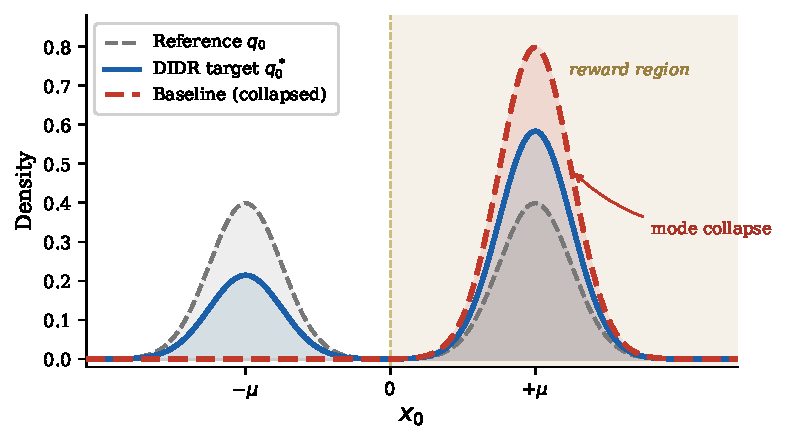
\includegraphics[width=\linewidth]{pictures/reward_domination.pdf}
  \caption{\textbf{Theoretical prediction} (\S\ref{subsec:trd}, $\tau=1$): $\mathcal{L}_{\mathrm{term}}$ collapses onto the rewarded mode (red) while $q^*$ remains a soft mixture (blue).}
\end{subfigure}
\hfill
\begin{subfigure}[t]{0.48\linewidth}
  \centering
  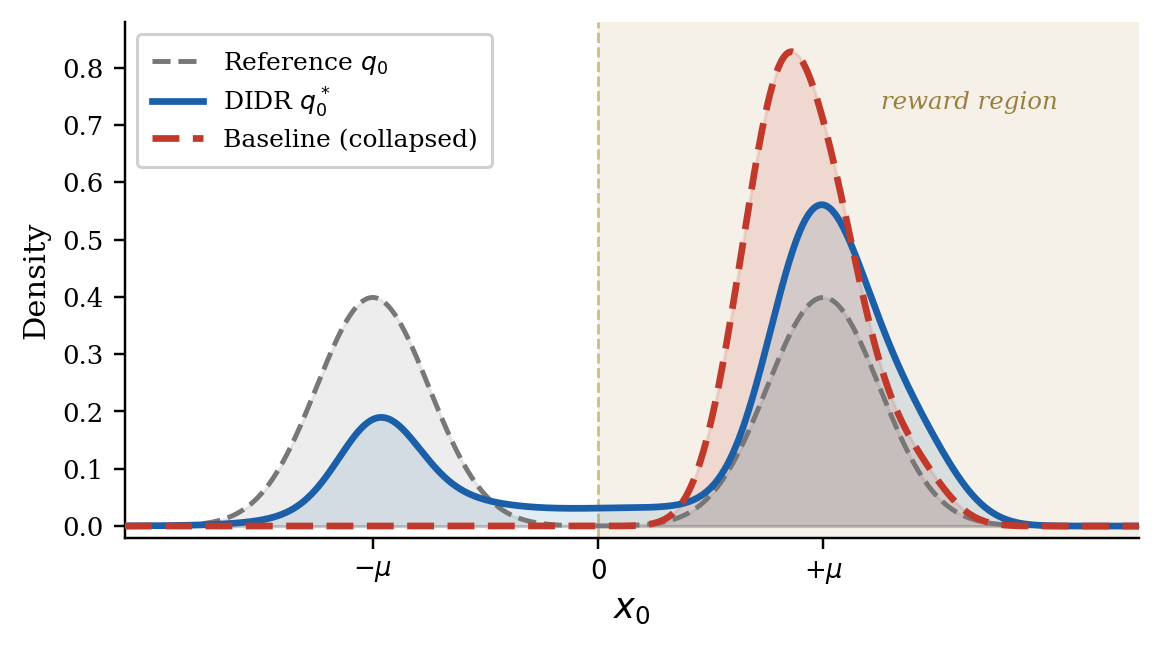
\includegraphics[width=\linewidth]{pictures/toy_1d_experiment.png}
  \caption{\textbf{1-D empirical validation} (setup in Appendix~\ref{app:toy_experiment}): \textsc{Didr} vs.\ DI++ as the baseline.}
\end{subfigure}
\vspace{-0.05in}
\caption{\textbf{Terminal reward domination.} The reward signal in $\mathcal{L}_{\mathrm{term}}$ tends to dominate the KL regularizer, causing the optimizer to over-tilt toward the high-reward mode relative to the balanced RLHF target $q^*$. \textbf{(a)} plots the theoretical prediction from \S\ref{subsec:trd}; \textbf{(b)} shows the 1-D empirical result (Appendix~\ref{app:toy_experiment}), confirming the collapse in practice even at $\tau=1$.}
\label{fig:schematic_combined}
\vspace{-0.1in}
\end{figure}

\subsection{Reward-Tilted Trajectory Objective}
\label{subsec:target}
Our core construction is the reward-tilted trajectory $\{q_t^*\}$, a principled optimization target defined at every noise level. We obtain it by lifting the RLHF optimum $q^*(x_0|c)$ (Eq.~\eqref{eq:reward_tilted_target}) to all noise levels via the reference forward process:
\begin{equation}
q_t^*(x_t|c)
=
\int q_t(x_t|x_0)\,q^*(x_0|c)\,\diff x_0 .
\label{eq:qt_star}
\end{equation}
The family $\{q_t^*\}_{t\in[0,T]}$ is the diffusion trajectory of the RLHF minimizer $q^*$, providing a well-defined target at every noise level. Proposition~\ref{thm:ikl_equiv} establishes the formal equivalence.

\begin{figure}[!t]
\vspace{-0.1in}
\centering
\begin{subfigure}[t]{0.48\linewidth}
  \centering
  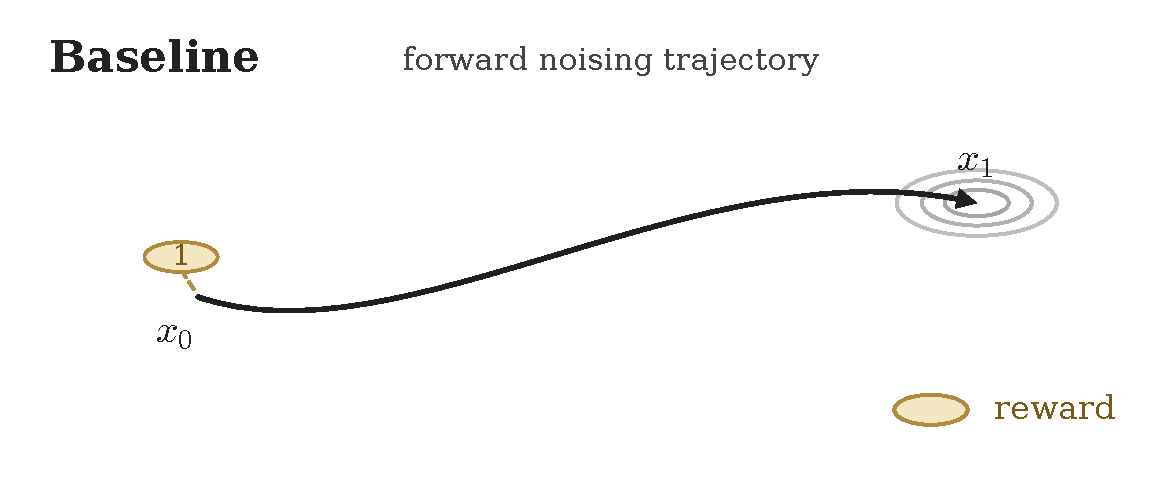
\includegraphics[width=\linewidth]{pictures/baseline_schematic.pdf}
  \caption{Terminal-reward alignment: reward only at $x_0$.}
\end{subfigure}
\hfill
\begin{subfigure}[t]{0.48\linewidth}
  \centering
  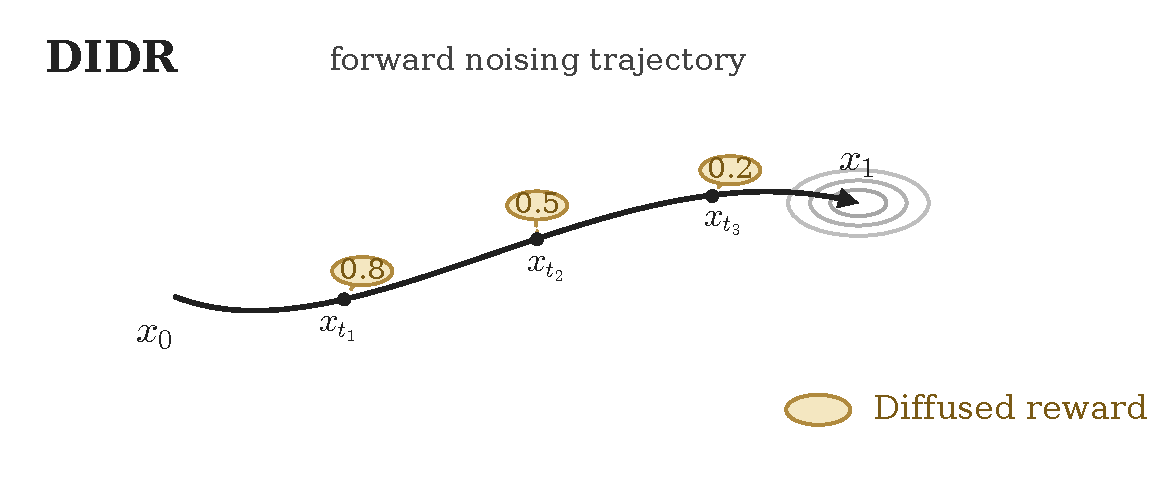
\includegraphics[width=\linewidth]{pictures/didr_schematic.pdf}
  \caption{\textsc{Didr}: reward at every $x_t$ via DRS.}
\end{subfigure}
\caption{\textbf{Reward propagation comparison.} Prior methods inject reward only at the clean endpoint $x_0$ while regularizing against bare reference marginals. \textsc{Didr} propagates preference through the full trajectory via the Diffused Reward Score.}
\label{fig:reward_comparison}
\end{figure}

\textbf{Objective.}
We train the generator by minimizing the IKL divergence between its forward-noised marginals $p_{\theta,t}$ and the reward-tilted trajectory $\{q_t^*\}$:
\begin{equation}
\mathcal{L}_{\mathrm{DIDR}}(\theta)
=
\E_{c\sim\mathcal{C}}
\left[
\int_0^T w(t)\,
\mathcal{D}_{\mathrm{KL}}\!\bigl(p_{\theta,t}(\cdot|c)\|q_t^*(\cdot|c)\bigr)\diff t
\right].
\label{eq:ikl_obj}
\end{equation}
By minimizing IKL against $q_t^*$ rather than the bare reference marginals, \textsc{Didr} encodes the full RLHF signal inside the trajectory without a separate terminal reward term, inheriting the broad distribution support and stable gradient flow of the IKL formulation while correctly injecting reward signals at every noise level.

\begin{proposition}[IKL shares the RLHF minimizer]
\label{thm:ikl_equiv}
For any clean distribution $p_0(\cdot|c)$ and its forward marginals $p_t(\cdot|c)$, if $Z(c)<\infty$ and $w(t)>0$ a.e., then
\[
\operatorname*{arg\,min}_{p_0}\mathcal{L}_{\mathrm{RLHF}}(p_0|c)
=
\operatorname*{arg\,min}_{p_0}\mathcal{L}_{\mathrm{DIDR}}(p_0|c)
=
\{q^*(\cdot|c)\}.
\]
\end{proposition}
(See Appendix~\ref{app:proof_thm_ikl_equiv} for proof.) The shared minimizer shows that the ideal IKL objective targets the RLHF optimum $q^*$. Note that this equivalence holds at the distribution level; the practical algorithm introduces score, posterior, and finite-sample approximations. Nevertheless, $\{q_t^*\}$ provides a well-defined optimization target throughout training.

\begin{theorem}[Score-based DIDR gradient]
\label{thm:score_gradient}
Differentiating the Integral KL through the generator and the forward noising process gives the ideal score-based gradient
\begin{equation}
\begin{aligned}
\nabla_\theta\mathcal{L}_{\mathrm{DIDR}}
=
\E_{\substack{c\sim\mathcal{C},\,z\sim p_z,\,t\sim\pi(t)\\
x_0=g_\theta(z,c)\\
x_t\sim q_t(\cdot|x_0)}}
\Bigg[
w(t)
\bigl(
s_\theta(x_t,t,c)
- s_{\mathrm{ref}}(x_t,t,c)
- s_r(x_t,t,c)
\bigr)
\frac{\partial x_t}{\partial\theta}
\Bigg].
\end{aligned}
\label{eq:ikl_grad}
\end{equation}
where $s_\theta(x_t,t,c)=\nabla_{x_t}\log p_{\theta,t}(x_t|c)$.
Also, $s_{\mathrm{ref}}(x_t,t,c)=\nabla_{x_t}\log q_t(x_t|c)$. The Diffused Reward Score (DRS) is
\begin{equation}
s_r(x_t,t,c)
=
\nabla_{x_t}\log
\E_{x_0\sim q(x_0|x_t,c)}
\left[
\exp\!\left(\frac{r(x_0,c)}{\tau}\right)
\right].
\label{eq:sr_definition}
\end{equation}
\end{theorem}
(See Appendix~\ref{app:proof_thm2} for proof.) The DRS term $s_r$ adds a reward-driven correction to the reference score, steering the generator toward the RLHF optimum at every noise level. Because $s_r$ is defined through the posterior $q(x_0|x_t,c)$, it propagates preference information only where the clean image is identifiable from the noisy observation, naturally attenuating reward guidance at high noise. The generator update is therefore driven by the mismatch between its own score and the reward-tilted target score $s_{\mathrm{ref}}+s_r$.

\begin{remark}[Connection to classifier guidance]
\label{rem:classifier_guidance}
Classifier guidance~\citep{dhariwal2021diffusion} is the first-order approximation of the DRS; the DRS keeps the full log-exponential tilt.
\end{remark}

\subsection{Diffused Reward Proxy}
\label{sec:drp}
Although the DRS provides a principled reward signal at every noise level, computing Eq.~\eqref{eq:sr_definition} requires the posterior $q(x_0|x_t,c)$, which is unavailable in closed form for a learned diffusion model. Assuming posterior samples admit a reparameterization $x_0 = \mathcal{G}(x_t,\boldsymbol{\epsilon},c)$ differentiable in $x_t$, differentiating the log-normalizer yields the pathwise form
\begin{equation}
\begin{aligned}
s_r(x_t,t,c)
=
\E_{x_0\sim q(x_0|x_t,c)}
\left[
\frac{\exp\!\left(\frac{r(x_0,c)}{\tau}\right)}
{\E_{\tilde{x}_0\sim q(\tilde{x}_0|x_t,c)}
\left[\exp\!\left(\frac{r(\tilde{x}_0,c)}{\tau}\right)\right]}
\cdot
\frac{1}{\tau}\nabla_{x_t}r(x_0,c)
\right],
\end{aligned}
\label{eq:drs_pathwise}
\end{equation}
where $\nabla_{x_t}r(x_0,c)$ is the gradient through a posterior sample $x_0$ treated as a function of $x_t$: the DRS is a reward-softmax-weighted average of pathwise reward gradients. We make this tractable by approximating the unavailable posterior with differentiable short-step denoising chains from $x_t$ under the frozen reference model, $\hat{x}_0 = \mathcal{G}_{\mathrm{ref}}(x_t,\boldsymbol{\epsilon},c)$, giving DRP formalized below.

\begin{proposition}[Diffused Reward Proxy]
\label{prop:drp}
Let $\hat{x}_0^{(k)}$ be $K$ independent $S$-step denoising samples from the frozen reference model,
\begin{equation}
\hat{x}_0^{(k)}
=
\mathcal{G}_{\mathrm{ref}}(x_t,\boldsymbol{\epsilon}^{(k)},c),
\qquad
k=1,\ldots,K,
\qquad
\boldsymbol{\epsilon}^{(k)}\sim p(\boldsymbol{\epsilon}) .
\end{equation}
For fixed $\boldsymbol{\epsilon}$, each chain is differentiable with respect to $x_t$. The DRP approximates the unavailable posterior expectation in Eq.~\eqref{eq:drs_pathwise} by the Monte Carlo estimator
\begin{equation}
\widehat{s}_r(x_t,t,c)
=
\frac{1}{\tau}
\sum_{k=1}^K
\omega^{(k)}
\nabla_{x_t}r(\hat{x}_0^{(k)},c),
\qquad
\omega^{(k)}
=
\frac{\exp(r(\hat{x}_0^{(k)},c)/\tau)}
{\sum_j \exp(r(\hat{x}_0^{(j)},c)/\tau)} .
\label{eq:drp_estimator}
\end{equation}
Here the pathwise reward gradient is
\begin{equation}
\nabla_{x_t}r(\hat{x}_0^{(k)},c)
=
\left(
\frac{\partial \mathcal{G}_{\mathrm{ref}}(x_t,\boldsymbol{\epsilon}^{(k)},c)}
{\partial x_t}
\right)^{\!\top}
\nabla_{\hat{x}_0}r(\hat{x}_0^{(k)},c).
\end{equation}
\end{proposition}
(See Appendix~\ref{app:proof_lem4} for derivation.) The softmax weights $\omega^{(k)}$ concentrate gradient mass on high-reward denoised images, while the pathwise Jacobian $\partial\mathcal{G}_{\mathrm{ref}}/\partial x_t$ propagates clean-image reward information back to $x_t$ through the frozen denoising chain without storing reference model activations.

\begin{remark}[Why the proxy works]
At low noise, the posterior $q(x_0|x_t,c)$ is concentrated, so short denoising chains yield accurate proxies. At high noise, $x_t$ carries little information about $x_0$, so the DRS correction is less sensitive to the accuracy of individual posterior samples; a short denoising proxy captures the leading-order correction.
\end{remark}

\vspace{-3mm}
\subsection{Practical Training with a Teaching Assistant}
\label{subsec:algorithm}
\vspace{-3mm}
Two substitutions make Eq.~\eqref{eq:ikl_grad} implementable. First, the generator score $s_\theta = \nabla_{x_t}\log p_{\theta,t}$ is unavailable for an implicit one-step generator; following~\citet{Luo2023DiffInstructAU}, we surrogate it with a Teaching Assistant (TA) score model $s_\psi$ trained concurrently via denoising score matching (DSM)~\citep{vincent2011connection,song2021scorebased} on noisy generator samples, so that $s_\psi(x_t,t,c)\approx s_\theta(x_t,t,c)$. Second, for text-to-image generation we replace the reference score $s_{\mathrm{ref}}$ with the CFG-corrected score
\begin{equation}
\tilde{s}_{\mathrm{ref}}(x_t, t, c) = s_{\mathrm{ref}}(x_t, t, \emptyset) + \cfg \bigl[ s_{\mathrm{ref}}(x_t, t, c) - s_{\mathrm{ref}}(x_t, t, \emptyset) \bigr],
\label{eq:cfg}
\end{equation}
where $\cfg\geq 1$ amplifies the prompt-conditional component.

\begin{remark}[Implicit and explicit reward signals]
The CFG-corrected reference score $\tilde{s}_{\mathrm{ref}}$ can be viewed as an implicit reward-tilted score induced by text guidance, while the DRS $s_r$ is an explicit correction from the chosen reward model. These two signals are complementary and can be combined, giving \textsc{Didr} flexibility in the reward design.
\end{remark}

With these substitutions, the practical generator update is
\begin{equation}
\operatorname{Grad}(\theta)
=
\E_{\substack{c\sim\mathcal{C},\,z\sim p_z,\,t\\
x_0=g_\theta(z,c),\,x_t\sim q_t(\cdot|x_0)}}
\left[
w(t)
\left(
s_\psi(x_t,t,c)
-
\tilde{s}_{\mathrm{ref}}(x_t,t,c)
-
s_r(x_t,t,c)
\right)
\frac{\partial x_t}{\partial\theta}
\right].
\label{eq:grad_practical}
\end{equation}

\textsc{Didr} alternates two stages (Algorithm~\ref{alg:didr}, Figure~\ref{fig:workflow}). \textbf{Stage I} keeps $s_\psi$ synchronized with the evolving $g_\theta$: sample $x_0 = g_\theta(z,c)$, diffuse to $x_t$, and update $s_\psi$ via DSM. \textbf{Stage II} updates $g_\theta$: draw $K$ differentiable $S$-step denoising chains from $x_t$, compute the DRP weights, and backpropagate Eq.~\eqref{eq:grad_practical} to $\theta$. Both the reference diffusion model and the reward model remain frozen throughout.

\vspace{-3mm}
